\documentclass[conference]{IEEEtran}
\usepackage{graphicx}
\usepackage{float}
\usepackage{amsmath}
%\usepackage{cite}

\begin{document}

\title{Direction of Angle Estimation}

\author{\IEEEauthorblockN{Owen Sowatzke}
\IEEEauthorblockA{\textit{Electrical Engineering Department} \\
\textit{University of Arizona}\\
Tucson, USA \\
osowatzke@arizona.edu}}
\maketitle

\begin{abstract}
	Direction of arrival (DOA) estimation plays an integral role in radar, wireless communications, sonar, radio astronomy, and navigation \cite{doa_algorithms_raghu}. Specific algorithms for DOA estimation include beamforming, MVDR, MUSIC, improved MUSIC, Root Music, and ESPRIT \cite{doa_algorithms_raghu}. Following the work of Raghu and Kamari, this paper evaulates the performance of each of these direction of arrival algorithms operating on data from a uniform linear array. 
\end{abstract}

	\section{Background}
	
	Each of the direction of angle algorithms compared in this report operate on data collected with an antenna array. This report specifically examines data collected with a uniform linear array (ULA). A block diagram of a uniform linear array with $M$ antenna elements, receiving signals from $D$ sources is given by Raghu and Kamari in \cite{doa_algorithms_raghu}.
	
	\begin{figure}[H]
		\centerline{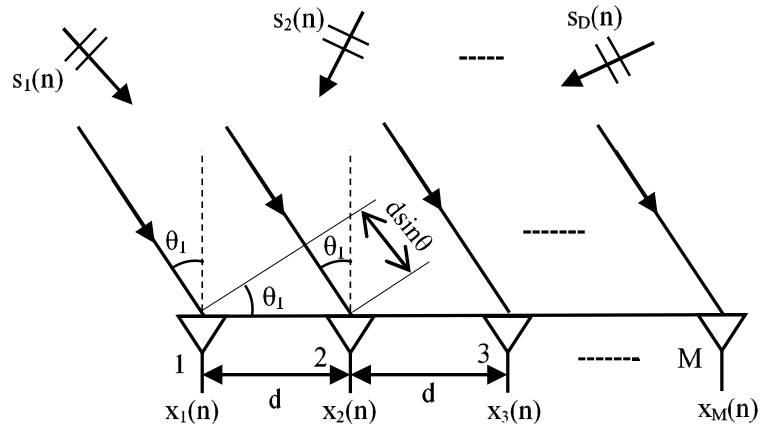
\includegraphics[width=0.5\textwidth]{uniform_linear_array.png}}
		\caption{Uniform Linear Array \cite{doa_algorithms_raghu}}
		\label{Monte Carlo Estimate}
	\end{figure}
	
	As shown in the figure above, let $d$ be the distance between successive array elements, and $\beta$ be defined as $2\pi/\lambda$. Then if each of the source signals is given as $s_1(n),...,s_D(n)$, the received signal on the m-th element can be written as:
	%
	\begin{equation}
		\begin{split}
			x_m(n) &= s_1(n)e^{-j{\beta}d(m-1)\sin{\theta_1}} + \cdots\\
			&+ s_D(n)e^{-j{\beta}d(m-1)\sin{\theta_D}} + w_m(n)
		\end{split}
	\end{equation}
	%
	where $w_m(n)$ denotes the noise on the m-th element \cite{doa_algorithms_raghu}.
	
	\bibliographystyle{IEEEtran}
	\bibliography{IEEEabrv,sources}
\end{document}